\section{Storage}

\framedt{Data Loss}{
   \textit{``Storage is crucial because, if a switch fails, or a server fails, the service will be interrupted, but the data will still be there. \ul{If the storage fails, the \textbf{data will be lost}}.''}
   -Prof. Cisternino\\

   \textbf{Data} is the most important of a system. Since data loss is \textbf{permanent}, the storage is completely different from computing or networking.
}

\begin{paracol}{2}
   
   Historically the storage was the slowest part of the system, \textit{ms} against \textit{ns} of the CPU.
   Today, with SSDs, the gap is considerably reduced to \textit{us}.
   
   \ul{NVMe stands for \textit{Non-Volatile Memory Express}, and is a protocol (\textit{not a HW component!})} that allows to access the storage directly from the PCIe bus, without having to go through the SATA controller. This allows to have a much higher throughput, and a much lower latency.

   \note{Optane was a technology developed by intel which is now end of life}
   \switchcolumn

   \begin{figure}[htbp]
      \centering
      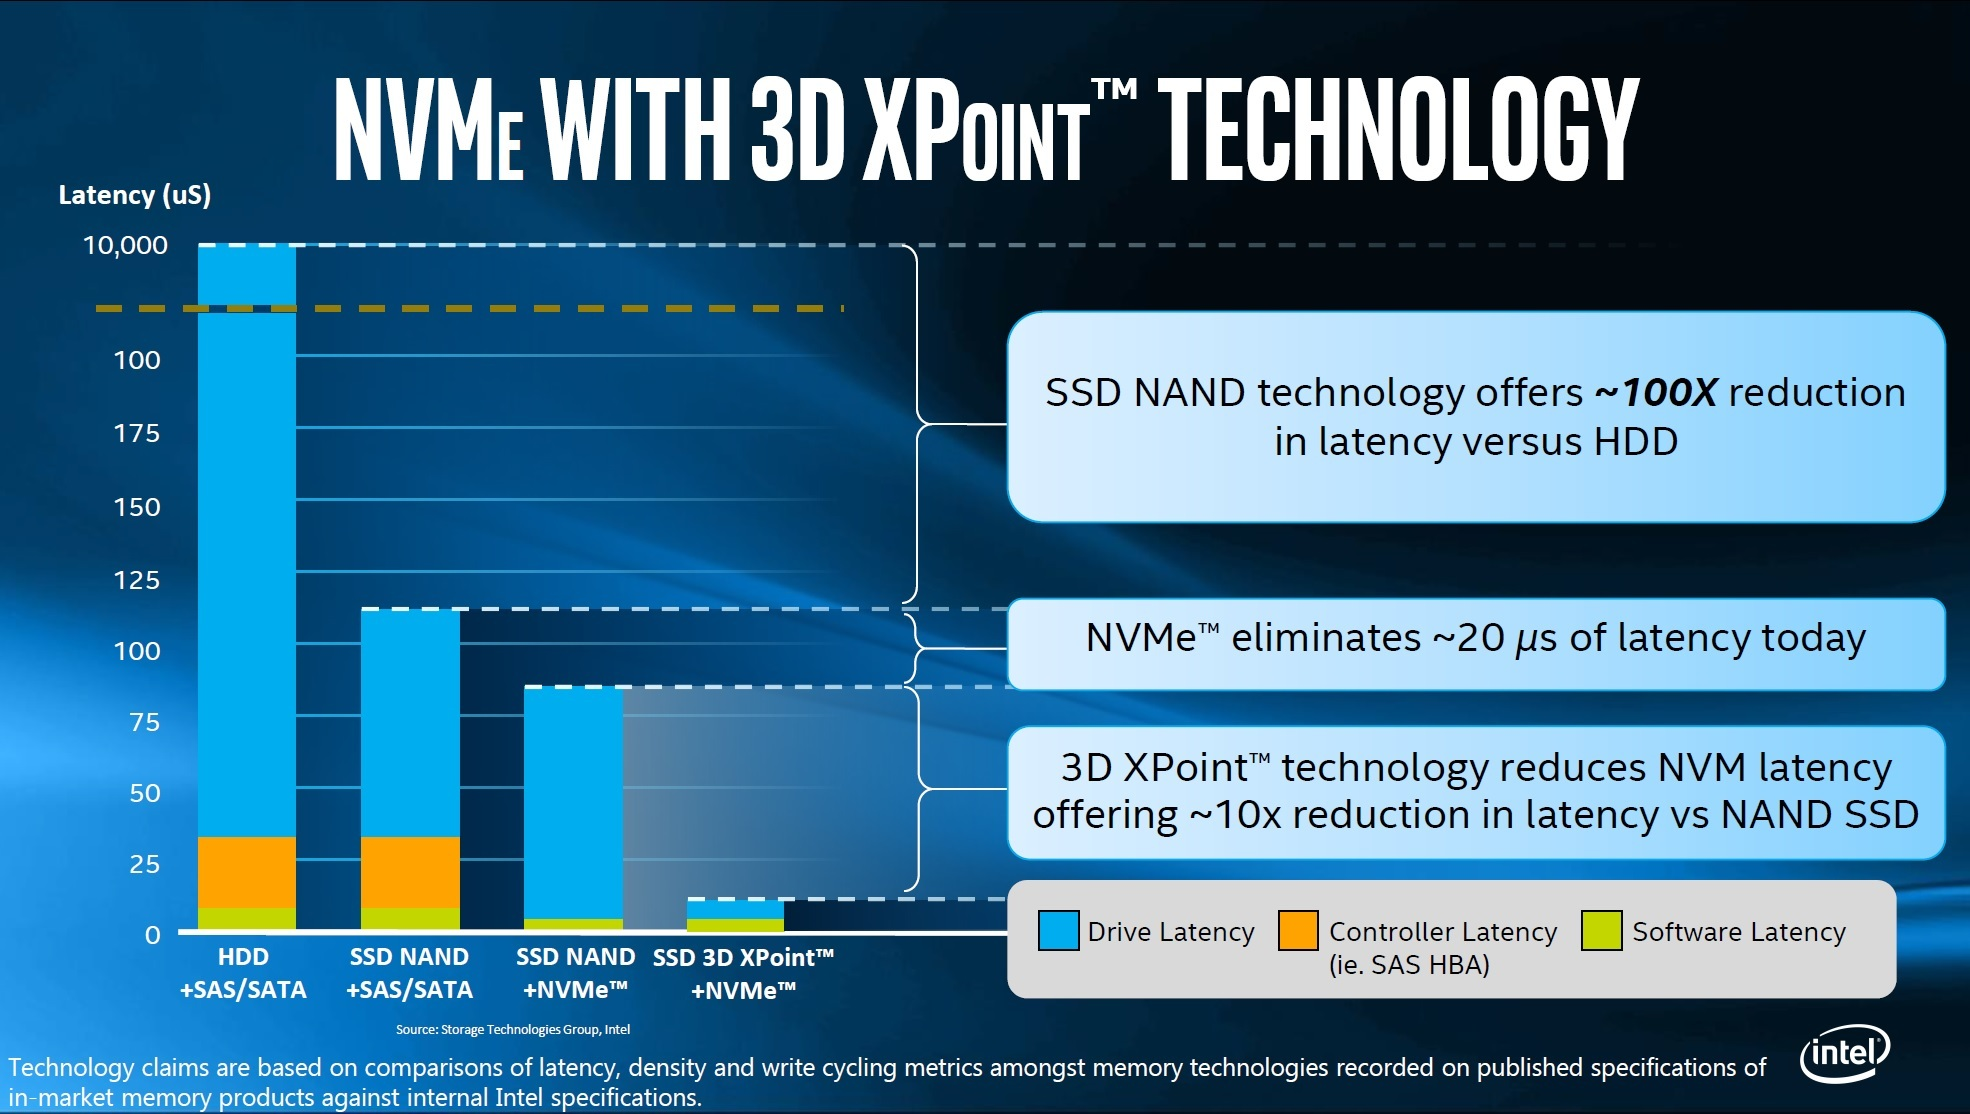
\includegraphics{images/storage_intel.jpg}
      \caption{Storage types comparison}
      \label{fig:storage_intel}
   \end{figure}
\end{paracol}

SSDs were invented by Toshiba back in 1980, but they were not popular for almost 30 years, until they eventually became cost-effective. Sometimes extra size in SSDs is used for redundancy, to increase the lifespan of the disk e.g. on a 30TB disk, only 10TB are used, the rest is used for redundancy, extending x3 the lifespan of the disk.

\begin{center}
   \textit{Why would a 15TB disk be better than a 27TB disk?}\\
   \note{Assume the same performance, and the same price.}
\end{center}
It would be preferrable because \ul{it would take less time to extract all the data from the disk}\footnote{i.e. taking advantage of the space provided}, since it is smaller.

However, large capacity drives are used for \textit{cold storage}, where the data is not accessed frequently, speed is not a priority, and even if the data is accessed, only a portion of the disk is needed at a time; in case of failure and thus needing to retrieve an entire backup, the time taken to retrieve the data is not a priority, since this ---hopefully--- happens only ``once''.

\section{SSDs - QLC and TLC}

TLC stands for \textit{Triple Level Cell}, and QLC stands for \textit{Quad Level Cell}. The difference between the two is the number of bits stored in each cell. The more bits stored in each cell, the cheaper the disk is, but the slower it is. The more bits stored in each cell, the more difficult it is to read and write the data, and the more difficult it is to keep the data stored in the cell.

Generally QLC disks are used for cold storage, while TLC disks are used for hot storage.
TLC in general is more reliable than QLC, has a longer lifespan and better performance, however they cost more.

\section{Latency}
A mechanical hard drive introduces 2.71\% of latency when reading, for instance, 40MB of data.  Optane can perform 416 accesses in the same time needed by a mechanical hard drive to perform 1 access. It looks like the latency in this latter case is neglegtible. Someone may be tempted to reduce the size of read/write operations and perform multiple smaller ones, since ``it's free''. 

\section{Checkpoints}
It's unpractical for a system to go down after 5 months. For this reason it is necessary to have checkpoints, which are points in time where the system can be restored to. The system can be restored to the last checkpoint, and the data that was written after the checkpoint can be re-applied. This is similar to what happens to applications on smartphones are closed and then re-opened, the application is restored to the last checkpoint.

\section{RAID}
\textbf{RAID} stands for \textit{Redundant Array of Independent Disks}. It is a technology that allows to combine multiple disks into a single logical unit, in order to increase the performance, the reliability, or both. There are different levels of RAID, each with different characteristics.

Historically \textit{Redundant Array of Inexpensive Disks}, because it was more common for disks to eventually fail, so RAID was the only countermeasure to this. Today, disks are more reliable, so RAID is used more for performance reasons.

In RAID, \textbf{XOR} is used to calculate the parity of the data. The parity is used to recover the data in case of a disk failure. The parity is calculated by XORing the data of the disks. The parity is stored on a separate disk, called the parity disk. The parity disk is used to recover the data in case of a disk failure.

\section{Network sharing}
\textbf{SMB/CIFS} is a protocol that allows to share files over the network. It is used by Windows, but it is also supported by Linux and MacOS. NFS is a protocol that allows to share files over the network, it is used by Linux and MacOS, but it is also supported by Windows.\\
NFS is faster than SMB, but it is also less secure. SMB is slower than NFS, but it is also more secure.

\textbf{NAS} instead are devices that are connected to the network, and that are used to store files. They are used to store files that are accessed by multiple users, and that need to be accessed from multiple devices. NAS devices are used to store files that are accessed by multiple users, and that need to be accessed from multiple devices. NAS devices are used to store files that are accessed by multiple users, and that need to be accessed from multiple devices.

\note{HBA stands for \textit{Host Bus Adapter}, and is a device that allows to connect a computer to a storage device. It is used to connect a computer to a storage device, and to allow the computer to access the storage device.}

When we talk about \textbf{capacity}, there are two measures which we can refer to:
\begin{enumerate}
   \item \textit{Scale-\textbf{up}}:
   adding more disks to the same server
   \item \textit{Scale-\textbf{out}}:
   adding more servers to the same network
\end{enumerate}

SAN stands for \textit{Storage Area Network}, and is a network that is used to connect multiple storage devices to multiple servers. It is used to connect multiple storage devices to multiple servers, and to allow the servers to access the storage devices. It is used to connect multiple storage devices to multiple servers, and to allow the servers to access the storage devices.\\
SAN was, before SSDs, one of the datacenter pillars.
Its architecture included a ``Head'' to which drives were attached, and the head was connected to the network. The head was used to manage the drives, and to allow the servers to access the drives.\\
When SSDs became popular, the head became a bottleneck, because it was not able to keep up with the speed of the SSDs(Recall that 4 SSDs are enough to saturate a 10Gbit link, See Sec. \ref{sec:bandwidth_storage}). For this reason, the head was removed, and the drives were connected directly to the network. This is called \textbf{DAS}. 

\subsection{Synchronization Software and its Price}

The ``storage guy'' must ensure that there is no condition under which can happen data loss, because it is never an option. It is also important to have powerful \textbf{synchronization algorithms}, which must allow data to be copied and synchronized in multiple locations without disrupting performance and handling concurrency;
such software is typically \textit{costful}.

It is difficult nowdays to establish what is the ``right'' price for software. The shift from highly specialized and costful hardware to general hardware-plus-software, gave the software, which still a non-physical entity, increasingly more value, perhaps even too much.

\section{Snapshots, Compression and other features}
\subsection{Storage Provisioning}
Storage provisioning is the process of assigning storage to a server. It is used to assign storage to a server, and to allow the server to access the storage.
To decide how much storage to assign to a server, usually the architect overbooks the storage, even beyond an estimation of how much storage it will need in the future.

Besides, \ul{available space may \textit{decrease} over time.}
\textbf{Snapshots} are to blame in this case. Snapshots consists in saving the differences between the current state of the data and the previous state of the data. This allows to recover the \textit{overwritten} data in case of a failure, but it also takes up space. The more snapshots are taken, the more space is taken up. The more space is taken up, the less space is available for the data.

\subsection{Compression}
Compression grants less space to be used, but it also requires more CPU power. However note that also allows to save some \textbf{bandwidth}, which we know to be critical.
\textit{Searching} in compressed data is not trivial, but there are tools to do it, such as the \href{https://en.wikipedia.org/wiki/FM-index}{\texttt{FM-index}}.

\subsection{Pools and LUNs}

\textbf{Storage pools} 
are used to combine multiple storage devices into a single logical unit, in order to increase performance and reliability. 
\textbf{Storage LUNs} define a storage partition and are used to assign storage ---a portion of the pool--- to a server, and to allow the server to access the storage, using ACLs.

\texttt{SCSI} is a protocol whose idea is to create a BUS of drives to be accessed together. It is an old protocol, designed in 1979 for small computers, but it is still used today, because it is very reliable.
The key idea was for \ul{mutiple drives to share the same physical flat cable}.\\
It had been ``deprecated'' in favor of \texttt{NVMe}, but it is still used today, because it is very reliable.



\section{Hyperconverged Infrastructure}
SAN started to create a sensible bottleneck, so designers started to ``move drives towards the servers''.
\textbf{DAS} stands for \textit{Direct Attached Storage}, and is a technology that allows to connect multiple storage devices to a single server, in order to increase the performance, the reliability, or both.
The limitations is that you can only attach up to 2 or 3 drives to a server.

An idea came out to use the servers' internal drive to build a Storage Area Network, and this is called \textbf{VSAN}.

\textbf{HCI} stands for \textit{Hyperconverged Infrastructure}, and is a technology that allows to combine multiple servers into a single logical unit, in order to increase the performance, the reliability, or both. 
The idea was born to allow a scale-out architecture, where you can add more servers to the network.

The \textbf{Hypervisor} is the software that allows to run multiple virtual machines on a single server. There should be some locality between the VM and the storage, because the VM should be able to access the storage quickly.
\texttt{read} operations are always performed locally on local drives; \texttt{write} operations instead sometimes require to retrieve a remote piece of data.

\subsection{Riak}
Riak is a distributed database that is used to store data in multiple locations. 

Recently it has been recognized that \ul{using general purpose hardware is no longer a feasible option.}




